\documentclass[crop,tikz]{standalone}% 'crop' is the default for v1.0, before it was 'preview'
\usetikzlibrary{calc,positioning,shapes.geometric,backgrounds,fit,shadows.blur,arrows.meta}
\begin{document}
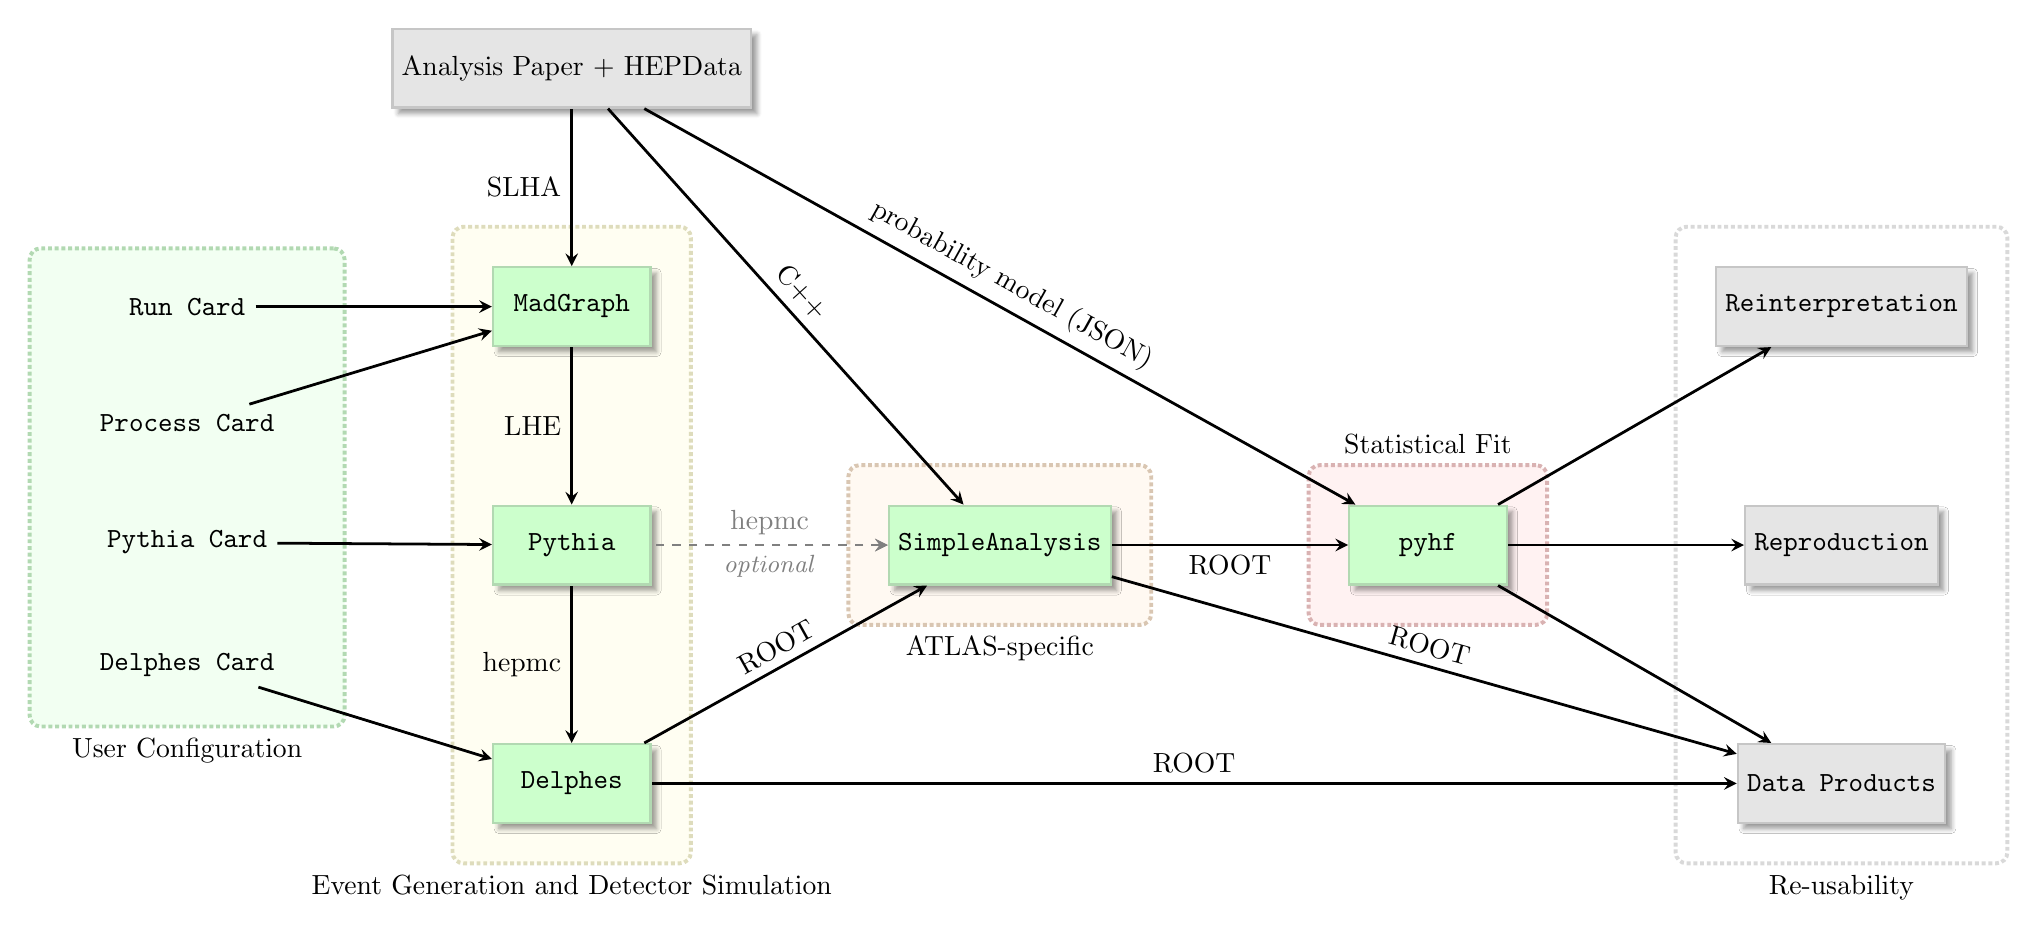
\begin{tikzpicture}[
		align=center,
		>=stealth,
		node distance=4cm,
		auto,
		line width=0.3mm,
		colorit/.style={
				draw=#1!50!black!30,
				fill=#1!20,
				thick,
				blur shadow={shadow blur steps=5}
			},
		colorit/.default=black,
		tool/.style={rectangle,colorit=green, minimum height=1cm, minimum width=2cm},
		output/.style={rectangle,colorit=gray, minimum height=1cm, minimum width=2cm},
		boxit/.style={
				draw=#1!50!black!30,
				fill=#1!5,
				densely dotted,
				line width=0.5mm,
				rounded corners
			},
		boxit/.default=yellow
	]

	\node[output] (paper) at (0,0) {Analysis Paper + HEPData};
	\node[tool, below=2cm of paper] (madgraph) {\texttt{MadGraph}}
	edge [<-, line width=1.0pt] node[auto, align=center] {SLHA} (paper);
	\node[tool, below=2cm of madgraph] (pythia) {\texttt{Pythia}}
	edge [<-, line width=1.0pt] node[auto] {LHE} (madgraph);
	\node[tool, below=2cm of pythia] (delphes) {\texttt{Delphes}}
	edge [<-, line width=1.0pt] node[auto] {hepmc} (pythia);
	\node[tool, right=3cm of pythia] (simpleanalysis) {\texttt{SimpleAnalysis}}
	edge [<-, line width=1.0pt] node[auto, sloped] {ROOT} (delphes)
	edge [<-, line width=1.0pt] node[auto, sloped] {C++} (paper)
	edge [<-, line width=1.0pt, dashed, gray] node[auto, anchor=south] {hepmc} (pythia)
	edge [<-, line width=1.0pt, dashed, gray] node[auto, anchor=north] {\small\textit{optional}} (pythia);
	\node[tool, right=3cm of simpleanalysis] (pyhf) {\texttt{pyhf}}
	edge [<-, line width=1.0pt] node[auto] {ROOT} (simpleanalysis)
	edge [<-, line width=1.0pt] node[auto, sloped] {probability model (JSON)} (paper);
	\node[output, right=3cm of pyhf] (reproduction) {\texttt{Reproduction}}
	edge [<-, line width=1.0pt] node[auto] {} (pyhf);
	\node[output, above=2cm of reproduction] (reinterpretation) {\texttt{Reinterpretation}}
	edge [<-, line width=1.0pt] node[auto] {} (pyhf);
	\node[output, below=2cm of reproduction] (products) {\texttt{Data Products}}
	edge [<-, line width=1.0pt] node[auto] {} (pyhf)
	edge [<-, line width=1.0pt] node[auto, sloped] {ROOT} (delphes)
	edge [<-, line width=1.0pt] node[auto, sloped] {ROOT} (simpleanalysis);

	\node[left=3cm of madgraph] (runcard) {\texttt{Run Card}}
	edge [->, line width=1.0pt] node[auto] {} (madgraph);
	\node[below=1cm of runcard] (proccard) {\texttt{Process Card}}
	edge [->, line width=1.0pt] node[auto] {} (madgraph);
	\node[below=1cm of proccard] (pythiacard) {\texttt{Pythia Card}}
	edge [->, line width=1.0pt] node[auto] {} (pythia);
	\node[below=1cm of pythiacard] (delphescard) {\texttt{Delphes Card}}
	edge [->, line width=1.0pt] node[auto] {} (delphes);

	\begin{scope}[on background layer]
		\node [label={below:User Configuration}, minimum width=4cm, inner sep=0.5cm, boxit=green, fit=(runcard) (proccard) (pythiacard) (delphescard)] {};
		\node [label={below:Event Generation and Detector Simulation}, inner sep=0.5cm, boxit, fit=(madgraph) (pythia) (delphes)] {};
		\node [label={below:ATLAS-specific}, inner sep=0.5cm, boxit=orange, fit=(simpleanalysis)] {};
		\node [label={above:Statistical Fit}, inner sep=0.5cm, boxit=red, fit=(pyhf)] {};
		\node [label={below:Re-usability}, inner sep=0.5cm, boxit=white, fit=(reproduction) (reinterpretation) (products)] {};
	\end{scope}
\end{tikzpicture}
\end{document}
